\documentclass[9pt,twocolumn,twoside]{pnas-new}

\templatetype{pnasresearcharticle}

\title{Analysis of GitHub: A Online Social Network of Software Developers}

\author[a,1]{Austin James Hockenberry}

\affil[a]{Undergraduate Student at the State University of New York at Buffalo}

\leadauthor{Hockenberry}

\significancestatement{GitHub forms an online social community of developers. Understanding GitHub provides a window into how cooperation is structured and functions in the software development field. Deriving this information could advance the career of future software developers/engineers and company recruitment through understanding how the new connections are formed in this field. This research seeks to accomplish this task by analyzing key proprieties of a large sample dataset of developers on GitHub. I found that developer world is a small world where developers tend to form closely-knit, but open communities. I found that famous and well-connected developers tend to become rich and rich with more connections as more developers join GitHub. 
}

\authorcontributions{All work was completed by Austin Hockenberry.}
\authordeclaration{There should be no competing interests.}
\correspondingauthor{\textsuperscript{1}To whom correspondence should be addressed. E-mail: ajhocken@buffalo.edu}

\keywords{Network Science $|$ Social Networks $|$ Online Social Networks $|$ Software Development $|$ GitHub $|$ Internet $|$ Small World $|$ Preferential Attachment ...}

\begin{abstract}

Social networks are networks involving social actors. Social networks are so ubiquitous because our modern society can't function without constant human social interactions. Every interaction among humans with other humans results in networks being formed whether we acknowledge it or not. Understanding how social networks work is fundamental to understanding how human cooperation functions in any field or area. As of 2022, GitHub is the popular website that hosts Git repositories. GitHub currently offers features that allow developers to follow each other on the website. Consequentially, this results in an online social network of developers being formed through these followership connections. Fundamental questions about social networks arise as a result of this formation. For example, is the GitHub a small world? Do developers preferentially attach to well-connected developers? How resilient is the network to developers leaving the platform? I hypothesized that the GitHub would be a small, but fragile, world where preferential attachment would exist among developers. A large sample dataset of 37,700 developers and 289,003 connections among them on GitHub that was collected by other authors was downloaded and used to serve as the candidate for this investigation. The dataset was processed and analyzed using the Python NetworkX library to extract and save key properties and structures about and in the network. I found, through these results, that there was significant evidence to suggest that my aforementioned hypothesizes about the network were true. This finding hints towards the universal truths about human interactions and the social networks they form. 

\end{abstract}

\dates{Published on \today}

\begin{document}

\maketitle
\thispagestyle{firststyle}
\ifthenelse{\boolean{shortarticle}}{\ifthenelse{\boolean{singlecolumn}}{\abscontentformatted}{\abscontent}}{}

\dropcap{A}Social network is any social structure involving social actors \cite{wikipediasocialnetwork}.  Social actors can, but aren't limited to: humans, animals, companies, and organizations. We are, by nature, social creatures. We have a desire and want to interact with other people. In fact, we must interact with another in order to survive and advance in our current society. In particular, modern large-scale software development requires communication and cooperation between software developers to succeed. This is because software development is a long, usually constantly continuing, time intensive, and complex process that no person today can muster on their own. Consequentially, social networks are formed and must be formed as developers interact with other developers to create and maintain software.

\subsection*{GitHub} GitHub is an internet hosting website launched in 2008 for Git repositories currently owned by Microsoft \cite{wikipediagithub}. According to Wikipedia, as of 2022, GitHub has 83 million developers, hosts 200 million total repositories, and at least 28 million public repositories \cite{wikipediagithub}. GitHub is the largest source code host as of 2022 \cite{wikipediagithub}. If someone is in the software development or computer science field, then said person uses or is at least aware of GitHub. You may be asking, why is GitHub interesting? GitHub is interesting because it is an example of popular platform where a social network of software developers currently resides and is easy to extract. GitHub forms a social network of developers that is easy to extract by offering a feature where users can create an account, star their favorite repositories, and can add follow other users similar to most other social media websites such as Twitter and Facebook. This paper will be analyzing this network using Python libraries in order to understand the properties and structure of the social network of developers on GitHub.

\subsection*{Git} But, what is Git? Git is a free and open source distributed version control software primarily used by programmers for collaborative software development \cite{wikipediagit}. Git was created by Linus Torvalds, the creator of the Linux kernel, for Linux kernel development in 2005 \cite{wikipediagit}. As of 2022, a survey says that upwards 93.9\% of developers use Git for version control for software development \cite{wikipediagit}. If someone is in the software development or computer science field, then said person uses Git for developing software or is at least aware of Git.

\subsection*{Motivations} I am a Computer Science major. I commonly use GitHub to host and contribute to my own personal projects. The CSE (Computer Science and Engineering) courses at UB (University at Buffalo) also use GitHub to host and track course student projects. Therefore, my main motivation for studying a GitHub network is because I am actively part of the network myself.  So, it naturally peaks my interest. Another motivation is that, since I will likely be a developer/software engineer when I graduate, I want to understand social networks among developers/software engineers because connections are important to landing jobs in this field. It is potentially easier to gain important connections in a network if you are aware of how it is structured. 

\subsection*{Objectives} This paper seeks to answer the following questions about the GitHub Network:

\begin{enumerate}
  \item What does the network look like?
  \item Do developers typically have a high or low degree of connections in the network?
  \item How resilient is the network to failures (developers or fellowships being removed)?
  \item Does the "6 degrees of separation" idiom (small world) hold true in the network?
  \item Are the most influential developers in the network the same ones who have a large amount of connections?
  \item Are already well-connected developers given preferential treatment?
  \item Do developers tend to form close-knit communities?
  \item Are there any islands or is the network completely connected?
  \item Does there exist clear hubs in the network? If so, to what degree do they exist?
\end{enumerate}

\subsection*{Hypothesizes} 

\subsection*{What does the network look like?}

I hypothesis that the network looks extremely dense to the point of not being easily visualizable without looking like a mess. I think this because the dataset is quite large both in terms of nodes and edges. It is often the case that networks that have large nodes and edges are hard to impossible to visualize.

\subsection*{Do developers typically have a high or low degree of connections in the network?}

I hypothesis that most developers will have a small degree of connections in the network. That is, the network will be very spare. I suspect this because in my experience, I tend to see that most people on GitHub only follow a couple of projects and people. I also speculate that there will be a couple of hubs (developers with large degrees) in the network. I believe that this will hold true because I know there are projects and people such as Linus Torvalds (original creator of Linux) with the Linux projects that most developers are aware of and follow. 

\subsection*{How resilient is the network to failures (developers or fellowships being removed)?}

I conjecture that there will be a small number of articulation points (single points of failures in the network that would disconnect it if removed) in the network. I believe that this will hold true because as I mentioned before, in my experience, most people on GitHub follow at least one of the key projects such as the Linux project on GitHub. Thus, it logically follows that there will usually be a way for other developers to stay connected through those hub projects.

\subsection*{Does the "6 degrees of separation" idiom (small world) hold true in the network?}

I surmise that the “6 degrees of separation” idiom this isn’t completely true, but I believe that it will be close. However, I am fairly certain that the social network will exhibit a clear small world property because the literature seems to suggest that “social networks are intuitive examples of this organization, in which cliques or clusters of friends being interconnected but each person is really only five or six people away from anyone else” \cite{PMC3604768}.

\subsection*{Are the most influential developers in the network the same ones who have a large amount of connections?}

I suspect that most influential developers in the network are the same ones with largest amount of connections. There is a common understanding that connections are powerful. Thus, my intuition tells me that the more connections a developer has, the influential they are, and vice versa.

\subsection*{Are already well-connected developers given preferential treatment?}

I suspect that yes, well-connected developers are given preferential treatment. Since GitHub is a social network, my intuition tells me that “rich will get richer” like most social networks. I commonly observe that the most popular developers only become more and more popular with time at a rate much greater than less popular developers.

\subsection*{Do developers tend to form close-knit communities?}

I believe this will hold true. This is because the literature seems to suggest that social networks tend to involve “cliques or clusters of friends being interconnected” \cite{PMC3604768}.

\subsection*{Are there any islands or is the network completely connected?}

I think it is likely that the network will be completely connected. As I mentioned, in my experience, most people on GitHub follow at least one of the key projects such as the Linux project on GitHub. Thus, if this true, the network would be completely connected.

\subsection*{Does there exist clear hubs in the network? If so, to what degree do they exist?}

I suspect that there will be very clear hubs in the network. As I mentioned, in my experience, most people on GitHub follow at least one of the key projects such as the Linux project on GitHub. Thus, these kinds of famous projects and people I believe will appear as clear hubs in the network.

\section*{Material and Methods}

\subsection*{Data Acquisition} A network dataset was download from the public network science repository SNAP as a zip file \cite{rozemberczki2019multiscale}. The dataset was originally collected by Benedek Rozemberczki, Carl Allen, Rik Sarkar using a public API for GitHub in June 2019 \cite{rozemberczki2019multiscale}. In the network, each node represents a developer who has starred at least 10 repositories and each edge represents a mutual follower relationship between two developers \cite{rozemberczki2019multiscale}. Vertex features were also extracted based on the location, repositories starred, employer, and e-mail address provided in the developer’s account on GitHub \cite{rozemberczki2019multiscale}. However, all the vertex features were disregarded for this analysis, since they weren’t used at all.

\subsection*{Data Processing} The raw dataset was processed by unzipping the archive and discarding all the files, but the CSV file named musae\_git\_edges.csv \href{https://github.com/Hockenba/mth450-final-project-report}{musae\_git\_edges.csv}. This CSV file contains the edge list representation of the network. The header of the aforementioned CSV file was also removed, since it was useless for parsing the file into a Python NetworkX Graph object for further more complex analysis. The CSV edge list representation of the network was converted into a NetworkX Graph Object with basic manually written code by myself and the Python CSV library. Python and the NetworkX library were selected for their ease of use, simplicity, vast variety of included functions for complex network analysis, and being ubiquitous within the Network Science field over other libraries and languages. The code used to perform the data processing is included in main.py \href{https://github.com/Hockenba/mth450-final-project-report}{main.py}.

\subsection*{Data Analysis} After the dataset was processed into a NetworkX Graph object, a variety of NetworkX functions were executed on the NetworkX Graph Object in order to extract different structures and properties of the GitHub network. Each type of different structure and property was created as a different process using the Python Multiprocessing library to allow greater throughout by levering the large multiprocessing performance of modern CPUs compared to their single process performance. The results of each process were saved as JSON file to avoid having to run the data analysis more than once, since most of these analyses took a long time to complete. The code used to perform the data analysis is included in main.py \href{https://github.com/Hockenba/mth450-final-project-report}{main.py}.

\subsection*{Data Visualization} After the information was analyzed and extracted from the network into a JSON file, then different processes were created to create any visualization. First, each process read its associated JSON file. Next, any visualizations such as pictorial figure/graphs were created and saved to PNG files at a specific path. In the case of raw single numbers, they were displayed to the terminal. In terms of libraries, Mathplotlib was used to generate the x-y graphs. Graphia was used to display the network. The code used to perform the data visualization is included in \href{https://github.com/Hockenba/mth450-final-project-report}{main.py}.

\section*{Results}

\subsection*{Network Visualization} The network itself is visualized in Figure \ref{fig:network_visualization}.

\begin{figure}
\centering
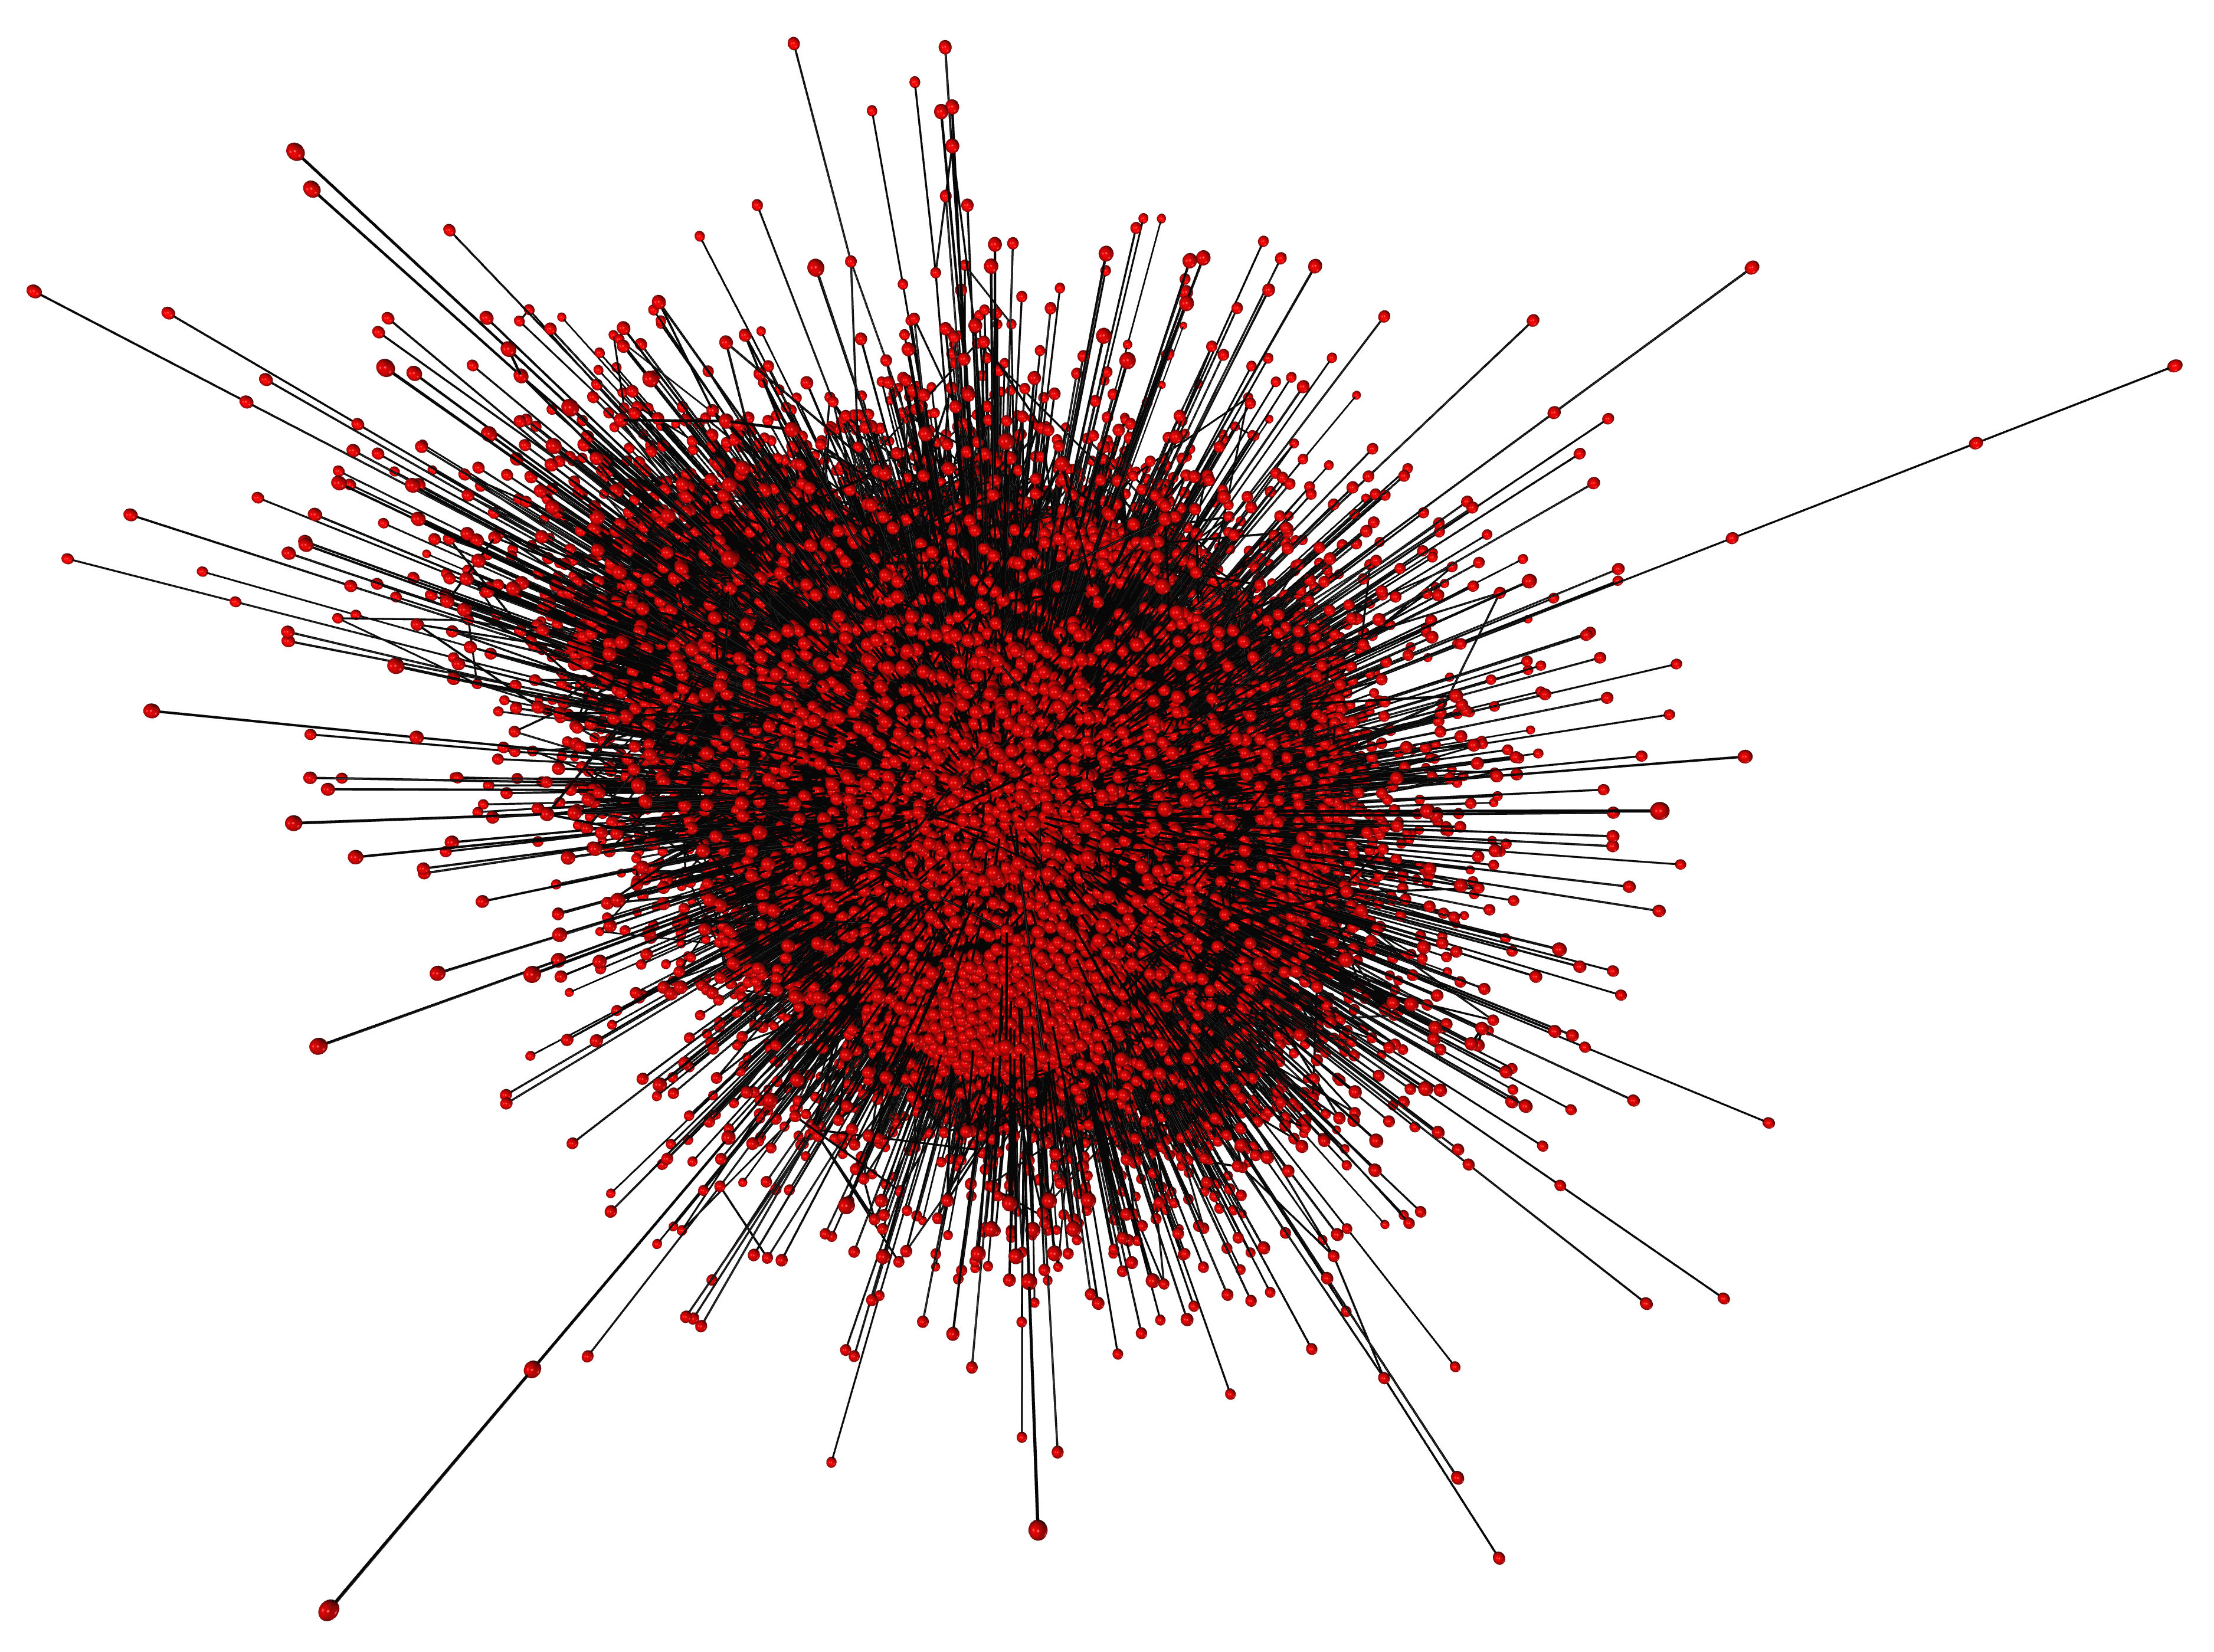
\includegraphics[width=.8\linewidth]{network_visualization}
\caption{Subgraph of the GitHub Followership Network as of June 2019. The nodes are in red and the edges are in black. All nodes and edges are the same size. Each node in the network is a developer who has starred at least 10 repositories. There is a total of 37,700 nodes and 289,003 edges in the network. Each edge is an undirected and unweighted edge denoting a mutual follower relationship between two developers who have at least starred 10 repositories. The network is completely connected.
}
\label{fig:network_visualization}
\end{figure}

\subsection*{Degree Frequency Histogram} The histogram of the degrees of the network is illustrated in Figure \ref{fig:degree_frequencies}.

\begin{figure}
\centering
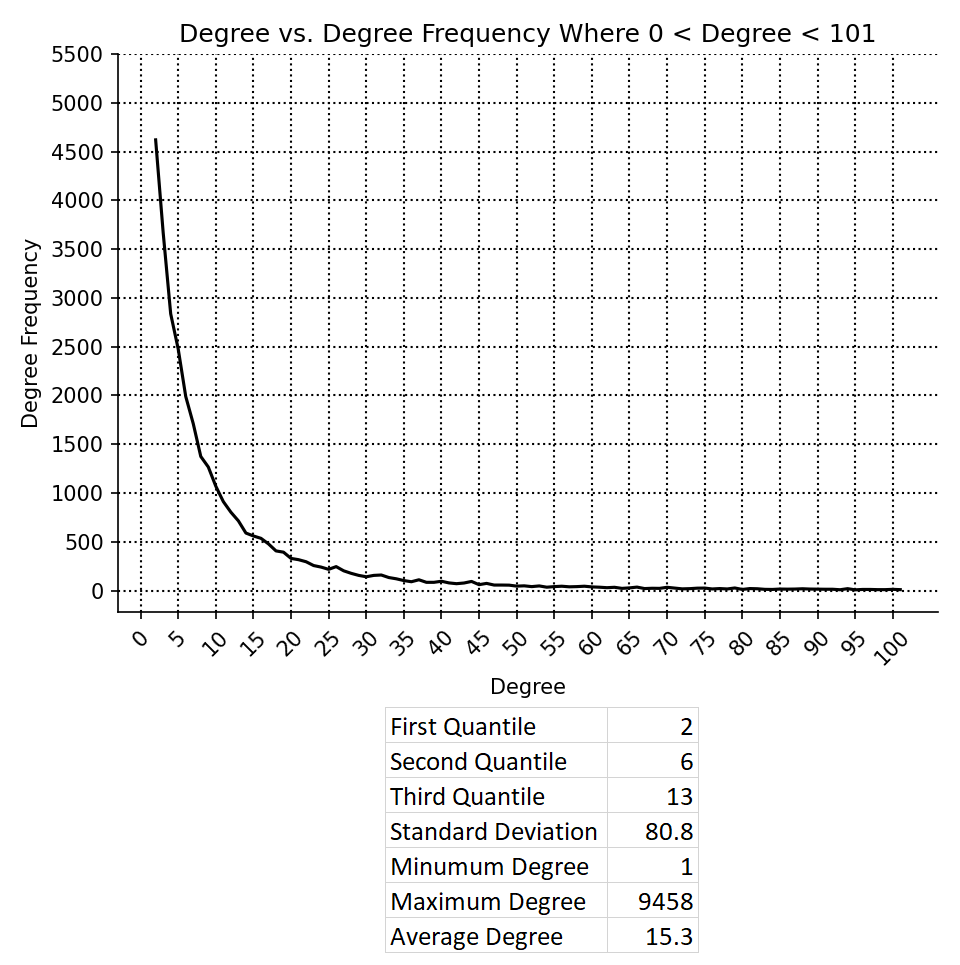
\includegraphics[width=.8\linewidth]{degree_frequencies}
\caption{The degree frequency distribution of the GitHub network where the degree is greater than 0 and less than 101. Degree 0 was included because there were no nodes with degree 0 and degrees above 100 also weren't included because all their frequencies were extremely small in comparison to smaller degree nodes. The degree of a node is the number of incident edges connected to said node. The embedded table gives some important statistics about the degrees of the network such as the 1-3 quantiles, median, standard deviation, minimum, and maximum degree of the network.
}
\label{fig:degree_frequencies}
\end{figure}

\subsection*{Rich Club Coefficients} The data involving the rich club coefficient of the network is included in Figure \ref{fig:rich_club_coefficients}.

\begin{figure}
\centering
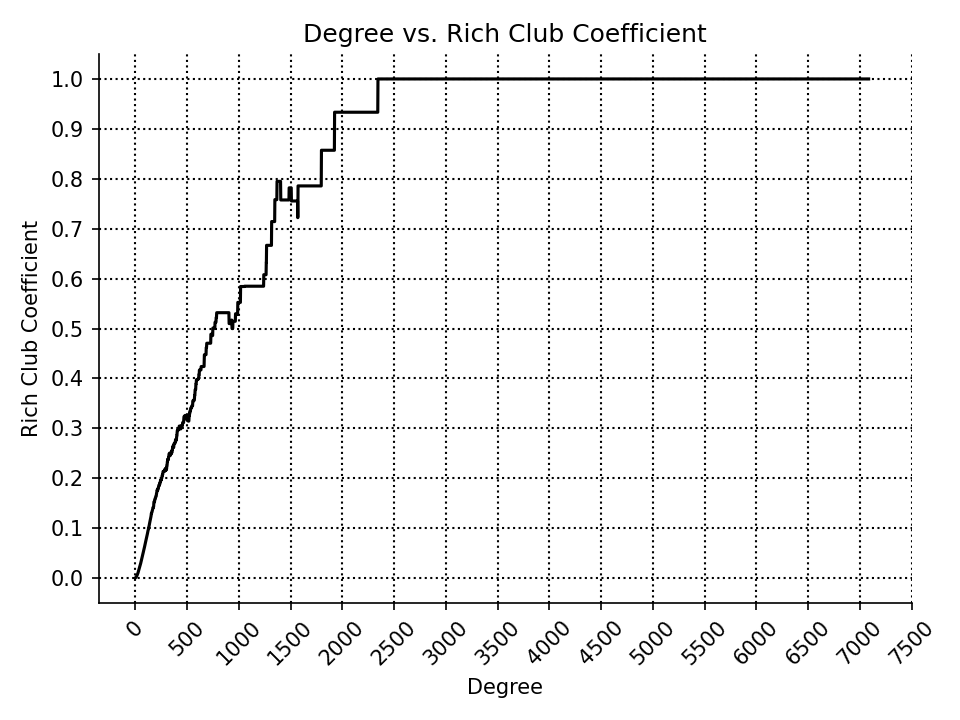
\includegraphics[width=.8\linewidth]{rich_club_coefficients}
\caption{The correlations between the degree of a node and its rich club coefficient within the sampled GitHub Network. The Rich Club Coefficient $\phi(k)$ is defined as $\phi(k)=\frac{2E_{k}}{N_{k}(N_{k} - 1))}$, where $N_{k}$ is the number of nodes with degree larger than \textit{k} and $E_{k}$ is the number of edges among those nodes \cite{networkxrichclubcoefficients}.
}
\label{fig:rich_club_coefficients}
\end{figure}

\subsection*{Density} The density \textit{d} of the network is defined as 
$d= \frac{2m}{n(n-1)}$
where \textit{m} is the number of edges in the network and \textit{n} is the number of nodes in the network \cite{networkxdensity}. The density of the GitHub network analyzed was $\approx 0.0004066878203117068$.

\subsection*{Articulation points} An Articulation point in a network is a node that if it and its edges were removed from the network, then the network would become disconnected. Hence, articulation points represent single point of failures in a network. The network has 3188 articulation points.

\subsection*{Diameter and Eccentricity} Commonly, the diameter of a network is the longest shortest path between any two nodes in the network. The eccentricity of a node (the diameter is the maximum of the eccentricities) is the longest shortest path from some said node to any other node in the network. In the first case, the diameter of the network is $11$, the average eccentricity starting at some node was $\approx 7.2286737400530505$, and the minimum eccentricity was $6$.

\subsection*{Ranking and RankVote} The results of the calcuation of the ranking values of the network are pictured in Figure \ref{fig:vote_ranks}.

\begin{figure}
\centering
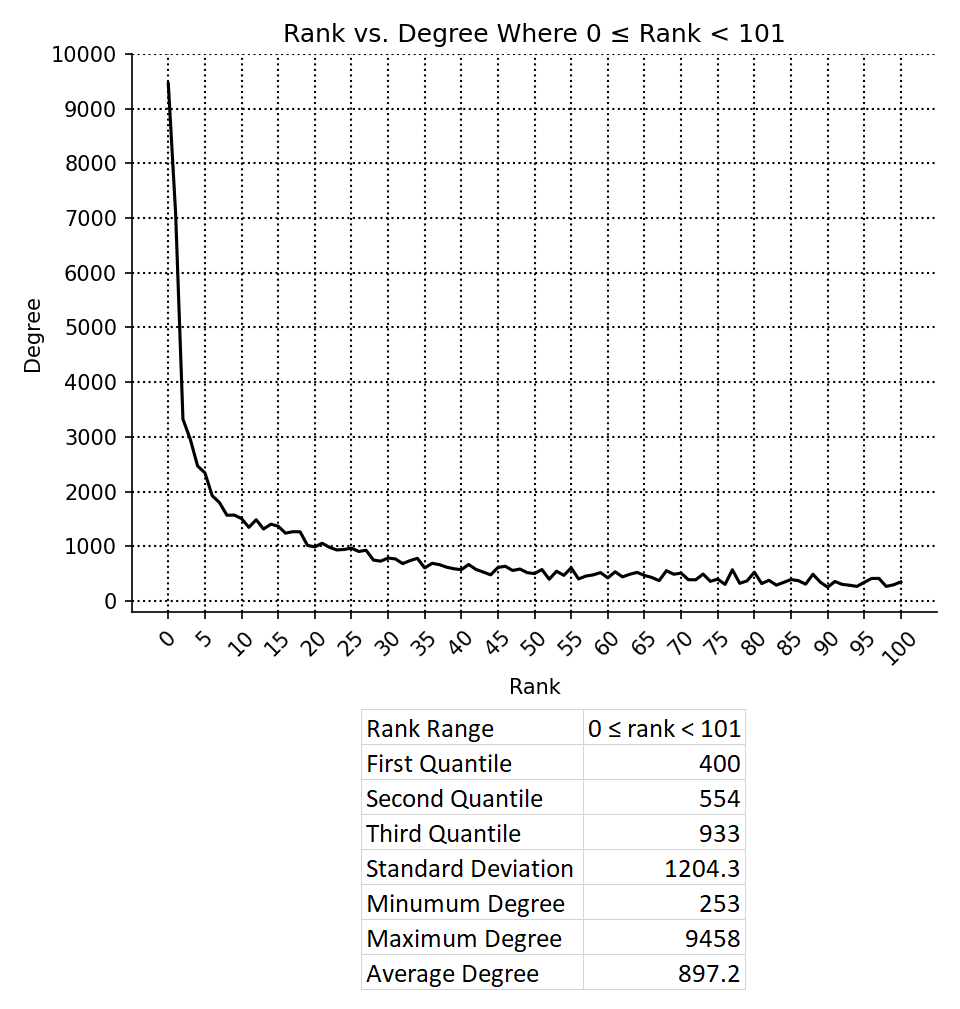
\includegraphics[width=.8\linewidth]{vote_ranks}
\caption{The ranking (x-axis) of the nodes compared to their degree (y-axis) where the rank is inclusively between 0 and 100. Smaller numbers correspond to greater rank while higher numbers correspond to lesser ranks. Only up to rank 100 was included because it would be impossible to visualize the rest of the ranks in one figure and the pattern should be obvious from the first 101 ranks. Ranking was determined using the VoteRank algorithm \cite{networkxvoteranks}.
}
\label{fig:vote_ranks}
\end{figure}

\subsection*{Closeness and Betweenness Centrality} The results of the calcuation of the closeness and betweenness centrality values of the network are pictured in Figure \ref{fig:centralities}.

\begin{figure}
\centering
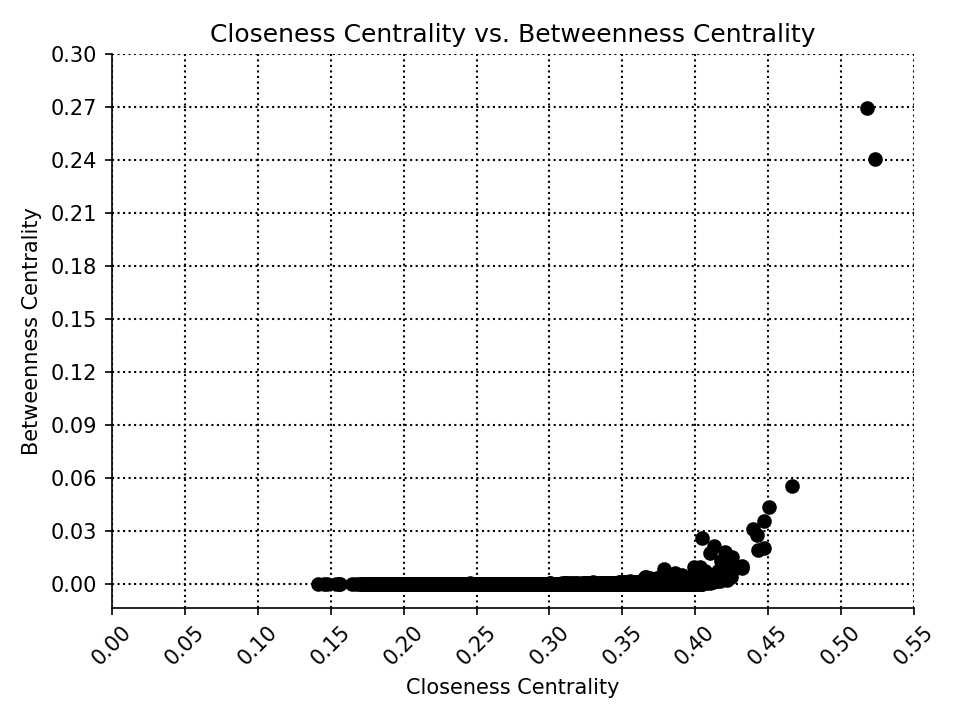
\includegraphics[width=.8\linewidth]{centralities}
\caption{A scatter plot of the closeness centrality (x-axis) to the betweenness centrality (y-axis) of the nodes in the network. The closeness centrality is defined as $C(u) =\frac{n-1}{\sum_{v=1}^{n-1}d(u, v)}$ \cite{networkxclosenesscentrality}. d(v, u) is the shortest-path distance between $v$ and $u$, and $n-1$ is the number of nodes reachable from $u$ \cite{networkxclosenesscentrality}. The betweenness centrality is defined as $e_{B}(v)=\sum_{s,t\in V}^{}\frac{\sigma(s, t|v)}{\sigma(s, t)}$ \cite{networkxbetweennesscentrality}. $V$ is the set of nodes, $\sigma(s, t)$ is the number of shortest $(s, t)$-paths, and $\sigma(s, t|v)$ is the number of those paths passing through some node $v$ other than $s, t$ \cite{networkxbetweennesscentrality}. 
}
\label{fig:centralities}
\end{figure}

\section*{Discussion/Conclusions}

\subsection*{What does the network look like?}

The network is visualized in Figure \ref{fig:network_visualization}. The network consists of a total of 37,700 nodes and 289,003 undirected edges. As hypothesized, The network is very complex to the point of being very hard to visualize. The network seems to have a very dense core of nodes with a lot of outlier nodes that connect the core. These outlier nodes seem to have a fairly low degree compared to the nodes in the core.

\subsection*{Do developers typically have a high or low degree of connections in the network?}

The degree histogram is pictured in Figure \ref{fig:degree_frequencies}. Looking at the degree histogram, we can conclude that most developers in the network on GitHub have an extremely small degree compared to the number of nodes in the network. The vast majority of developers have a degree less than even 13 compared to the possible maximum degree of 37,700. In fact, the density of the network is 0.0004066878203117068, which indicates that the network is actual very spare.

\subsection*{How resilient is the network to failures (developers or fellowships being removed)?}

We can conclude that the network is not very resilient to staying connected if some developer were to leave GitHub. This is because $\frac{3188}{37700} \approx$ 8.46\% of nodes represent single points of failure in the network. Around 8\% to 9\% may not seem like a lot, but if the network was disconnected in the future because of one of these articulation points, the effects could be extremely impactful to the rest network as a whole. People often meet new people and new projects through their existing connections. Think of all the time you have meet someone through a friend. Thus, if the network was disconnected in the future, it could lead to the two networks becoming isolated from one another. This could result in missed opportunities for recruitment and cooperation between developers, since two developers in each of the new disconnected subgraphs could have no preexisting connections to facilitate these new connections being formed. This additionally likely suggest that there are communities of developers that lie on the outside of the core of the network that is formed by the famous hub developers in the network.

\subsection*{Does the "6 degrees of separation" idiom (small world) hold true in the network?}

Yes and no. The "6 degrees of separation" idiom doesn't strictly hold because it was found that the diameter of the network was 11. However, arguably, it does suggest that idiom is good approximation of the idea that social networks are often highly interconnected. This is too the point that social actors in most social networks can easily trace back their connection to a any other social actor in a relatively small amount of steps compared to theoretical maximum. The theoretical maximum would simply just be $n-1$, where $n$ is the number of nodes in the network. However, this almost undeniably confirms that the network exhibits the small world property (diameter grows with O(log(n)) because $11 < \log_{2}\left(37700\right) \approx 15.2$. This is great because it confirms our hypothesis that the GitHub would have a structure similar to the most social networks, where the small world property is all too commonly known by even the common person.

\subsection*{Are the most influential developers in the network the same ones who have a large amount of connections?}

Yes, as conjectured, the most influential developers in the network are the same ones who have a large amount of connections in the network. We can draw this conclusion from Figure \ref{fig:vote_ranks}, where there is a clear trend where the top most influential developers have extraordinary large degrees compared to the rest of the network. This fundamentally demonstrates that the degree of a developer highly correlated with it influence over the network in this particular example.

\subsection*{Are already well-connected developers given preferential treatment?}

As hypothesized, Figure \ref{fig:rich_club_coefficients} undeniably demonstrates a upward trend in the rich club coefficient of a developer as the degree of said developer also increases. What we can extract from this finding is that, indeed, the well-connected developers are also well-connected to each other. Furthermore, we extrapolate from this conclusion to reasonable infer that the rich do get richer in the network. That is, our expectation that the network would follow general observations and understandings about social networks that the richly connected are given preferential treatment.

\subsection*{Do developers tend to form close-knit communities?}

Yes, it appears that developers tend to form close-knit communities. However, it also seems that they form close-knit communities that strongly connect to other close-knit communities. This observation can be derived from the the absurdly low betweenness centrality values and relatively high closeness values shown in Figure \ref{fig:centralities}. This is because the existence of this pattern of values suggest that most developers have lots of connections with developers that their neighbors also have connections with. Thus, illustrating that they all densely interconnected with one another, and thus aren't typically dependent on their neighbors to have a connection with close developers.

\subsection*{Are there any islands or is the network completely connected?}

As we can see from the description of Figure \ref{fig:network_visualization}, the network has no island because it is completely connected. That is, we can trace a path from any developer to any other developers. Combined with the absurdly low betweenness centrality values and relatively high closeness values shown in Figure \ref{fig:centralities}, this potentially alludes to the interconnectedness of interactions between developers. Furthermore, the observation that developers likely don't have a tendency to form exclusionary communities. Not forming exclusionary communities might hint towards the tendency of developers to value cooperativeness with new people outside of their usual clique of intimate relationships.

\subsection*{Does there exist clear hubs in the network? If so, to what degree do they exist?}

Looking at figure \ref{fig:degree_frequencies}, \ref{fig:vote_ranks}, \ref{fig:centralities}, we can easily reach the conclusion that there are clear hubs in the network. This is because there are a number of developers such as the developer with the maximum degree of 9458 and extraordinary centrality values such as the nodes in the top right of Figure \ref{fig:centralities}. This is in compared to most nodes that can barely reach 10 connections and centrality in the bottom portion of figure \ref{fig:centralities}. If we were to define a intuitive definition of the degree to which clear hubs exist as the one minus average degree over the maximum degree, we get a score $\frac{9458}{15.3} = \approx 618.169934641$. This articulates that the largest hub has a degree $\approx 618.169934641$ times greater than the average degree. Obviously, this shows that there are clearly famous or extraordinarily well-connected developers in the network compared to the rest of the developers. This fits our original assumption that these types of developers would exist because GitHub in a social network, where this phenomenon is extremely common. 

\subsection*{Opportunities for Future Research} Additional future research could be done on finding the exact communities, motifs, and effective size of the developers in the network. These types of analysis weren't included in this paper because they were too computationally intensive for my hardware to process in a reasonable timeframe (less than 24 hours of continuous runtime). By conducting these analyizes, larger patterns and insights into the interworkings of the network could be discovered.


\acknow{This research article was completed in Fall 2022 as part of graded course work for MTH 450: Network Theory at the State University of New York at Buffalo taught under Professor Dr. Naoki Masuda.
}

\showacknow{}

\section*{References}

\bibliography{pnas-sample}

\end{document}
